\chapter{Synchrotron Radiation}

%-----------------------------------------------------------------
\section{Synchrotron Radiation Damping and Excitation}
\label{s:radiation}
\index{synchrotron radiation!damping and excitation|hyperbf}

Emission of synchrotron radiation by a particle can be decomposed into
two parts. The deterministic average energy emitted produces damping
while the stochastic fluctuating part of the energy spectrum produces excitation\cite{b:jowett}.

\index{MAD!radiation}
The treatment of radiation damping by \bmad essentially follows \mad.
The average change in energy $\Delta E$ of a particle going through a
section of magnet due to synchrotron radiation is
\Begineq
  \frac{\Delta E}{E_0} = -k_d \, (1 + p_z)
\Endeq
where
\Begineq
  k_d \equiv \frac{2 \, r_e}{3} \, \gamma_0^3 \, \ave{g_0^2} \, L_p \,  
  (1 + p_z)
  \label{k2r3g}
\Endeq
$r_e$ is the classical electron radius, $L_p$ is the actual path
length, $\gamma_0$ is the energy factor of an on-energy particle, $1/g_0$
is the bending radius of an on--energy particle, and $\ave{g_0^2}$ is an
average of $g_0^2$ over the actual path.

The energy lost is given by
\Begineq
  \frac{\Delta E}{E_0} = -k_f \, (1 + p_z)
\Endeq
where
\Begineq
  k_f \equiv \left( \frac{55 \, r_e \, \hbar \, c}{24 \, \sqrt{3} \, m_e} \, 
  L_p \, \gamma_0^5 \ave{g_0^3} \right)^{1/2} \, (1 + p_z) \, \xi
  \label{k55rh}
\Endeq
$\xi$ is a Gaussian distributed random number with unit sigma and zero mean.

Using \Eqs{k2r3g} and \eq{k55rh} the total change in $p_z$ can be written as
\Begineq
  \Delta p_z = \frac{\Delta E}{E_0} = -k_E \, (1 + p_z)
\Endeq
where
\Begineq
  k_E = k_d + k_f
\Endeq
Since the radiation is emitted in the forward direction the angles
$x'$ and $y'$ are invariant which leads to the following equations for
the changes in $p_x$ and $p_y$
\begin{align}
  \Delta p_x &= -k_E \, p_x \CRNO
  \Delta p_y &= -k_E \, p_y 
\end{align}

The above formalism does not take into account the fact that radiation is 
emitted with a $1/\gamma$ angular distribution. This means that the calculated
vertical emittance for a lattice with
bends only in the horizontal plane and without any coupling elements such as
skew quadrupoles will be zero. Typically, in practice, the vertical emittance
will be dominated by coupling so this approximation is generally a good one.

%-----------------------------------------------------------------
\section{Synchrotron Radiation Integrals}
\label{s:synch.ints}
\index{synchrotron radiation!integrals}

The synchrotron radiation integrals are used to compute emittances,
the energy spread, etc. The standard formulas assume no coupling
between the horizontal and vertical planes\cite{b:helm,b:jowett}. With
coupling, the equations need to be generalized and this is detailed
below.

\index{dispersion}
In the general case, the curvature vector $\bfg = (g_x, g_y)$, which
points away from the center of curvature of the particle's orbit and
has a magnitude of $|\bfg| = 1/\rho$, where $\rho$ is the radius of
curvature (see \fig{f:local.coords}), does not lie in the
horizontal plane. Similarly, the dispersion $\bfeta\two =
(\eta_x, \eta_y)$ will not lie in the horizontal plane. With this
notation, the synchrotron integrals for coupled motion are:
  \begin{align}
    I_0 &= \oint ds \, \gamma_0 \, g \\
    I_1 &= \oint ds \, \bfg \dotproduct \bfeta 
         \equiv \oint ds \, (g_x \, \eta_x + g_y \, \eta_y) \\
    I_2 &= \oint ds \, g^2 \\
    I_3 &= \oint ds \, g^3 \\
    I_{4a} &= \oint ds \, \left[ g^2 \, \bfg \dotproduct \bfeta\two_a + 
         \nabla g^2 \dotproduct \bfeta\two_a \right] \\
    I_{4b} &= \oint ds \, \left[ g^2 \, \bfg \dotproduct \bfeta\two_b + 
         \nabla g^2 \dotproduct \bfeta\two_b \right] \\
    I_{4z} &= \oint ds \, \left[ g^2 \, \bfg \dotproduct \bfeta\two + 
         \nabla g^2 \dotproduct \bfeta\two \right] \\
    I_{5a} &= \oint ds \, g^3 \, \calH_a \\
    I_{5b} &= \oint ds \, g^3 \, \calH_b \\
    I_{6b} &= \oint ds \, g^3 \, \beta_b
  \end{align}
where $\gamma_0$ is that usual relativistic factor and $\calH_a$ is 
  \Begineq
    \calH_a = \gamma_a \, \eta_a^2 + 2 \, \alpha_a \, \eta_a \, \eta_a' + 
      \beta_a \eta_a'^2 
  \Endeq
with a similar equation for $\calH_b$. Here $\bfeta\two_a =
(\eta_{ax}, \eta_{ay})$, and $\bfeta\two_b = (\eta_{bx}, \eta_{by})$
are the dispersion vectors for the $a$ and $b$ modes respectively in
$x$--$y$ space (these 2--vectors are not to be confused with the
dispersion 4--vectors used in the previous section). The position
dependence of the curvature function is:
  \begin{align}
    g_x(x,y) = g_{x} + x \, k_1 + y \, s_1 \CRNO
    g_y(x,y) = g_{y} + x \, s_1 - y \, k_1 
  \end{align}
where $k_1$ is the quadrupole moment and $s_1$ is the skew--quadrupole moment.
Using this gives on--axis ($x = y = 0$)
  \Begineq
    \nabla g^2 = 2 \left( g_x k_1 + g_y s_1, \, g_x s_1 - g_y k_1 \right)
    \label{g2gkg}
  \Endeq

$I_0$ is not a standard radiation integral. It is useful,
though, in calculating the average number of photons emitted. For electrons:
  \Begineq
    {\cal N} = \frac{5 \: r_{\! f}}{2 \sqrt{3} \, \hbar \, c} \, I_0 
  \Endeq
where $\cal N$ is the average number of photons emitted by a particle
over one turn, and the ``classical radius factor'' $r_{\! f}$ is 
  \Begineq
    r_{\! f} = \frac{e^2}{4 \, \pi \, \epsilon_0} 
  \Endeq
$r_{\! f}$ has a value of $1.4399644 \cdot 10^{-9} \; \text{meters-eV}$
for all particles of charge $\pm 1$.

In a dipole a non--zero $e_1$ or $e_2$ gives a contribution to $I_4$
via the $\nabla g^2 \dotproduct \bfeta$ term. The edge field is modeled as a
thin quadrupole of length $\delta$ and strength $k = -\tan(e) /
\delta$. It is assumed that $\bfg$ rises linearly within the edge field
from zero on the outside edge of the edge field to its full value on the inside 
edge of the edge field. 
Using this in \Eq{g2gkg} and integrating over the edge field gives the contribution
to $I_4$ from a non--zero $e_1$ as
  \Begineq
    I_{4z} = -\tan(e_1) \, g^2
    \left( \cos(\theta) \, \eta_x + \sin(\theta) \, \eta_y \right)
    \label{iegct}
  \Endeq
With an analogous equation for a finite $e_2$. The extension to
$I_{4a}$ and $I_{4b}$ involves using $\bfeta\two_a$ and $\bfeta\two_b$
in place of $\bfeta\two$.  In \Eq{iegct} $\theta$ is the \vn{tilt}
angle which is non--zero if the bend is not in the horizontal plane.

The above integrals are invariant under rotation of the $(x,y)$ coordinate
system and reduce to the standard equations when $g_y = 0$ as they should.

There are various parameters that can be expressed in terms of these
integrals.  The $I_1$ integral can be related to the momentum
compaction $\alpha_p$ via
  \Begineq
    I_1 = \alpha_p \, L
  \Endeq
where $L$ is the storage ring circumference. The energy loss per turn is
  \Begineq
    U_0 = \frac{2 \, r_e E_0^4}{3 \, (mc^2)^3} I_2
  \Endeq
where $E_0$ is the nominal energy and $r_e$ is the classical electron
radius (electrons are assumed here but the formulas are easily
generalized).

The damping partition numbers are
  \Begineq
    J_a = 1 - \frac{I_{4a}}{I_2} \comma \quad
    J_b = 1 - \frac{I_{4b}}{I_2} \comma \, \text{and} \quad \label{j1ii}
    J_z = 2 + \frac{I_{4z}}{I_2} \period
  \Endeq
Since 
  \Begineq          
    \bfeta\two_{a} + \bfeta\two_{b} = \bfeta\two
    \comma \label{eee}
  \Endeq
Robinson's theorem, $J_a + J_b + J_z = 4$, is satisfied.
Alternatively, the exponential damping coefficients per turn are
  \Begineq
    \alpha_a = \frac{U_0 \, J_a}{2 E_0} \comma \quad
    \alpha_b = \frac{U_0 \, J_b}{2 E_0} \comma \, \text{and} \quad
    \alpha_z = \frac{U_0 \, J_z}{2 E_0} \period
  \Endeq
The energy spread is given by
  \Begineq
    \sigma_{pz}^2 = \left( \frac{\sigma_E}{E_0} \right)^2 = 
    C_q \gamma_0^2 \frac{I_3}{2I_2 + I_{4z}}
  \Endeq
where $\gamma_0$ is the usual energy factor and 
  \Begineq
    C_q = \frac{55}{32 \, \sqrt{3}} \, \frac{\hbar}{mc} = 
    3.84 \times 10^{-13} \, \text{meter for electrons}
  \Endeq
If the synchrotron frequency is not too large, the bunch length is given by
  \Begineq
    \sigma_z = \frac{I_1}{M(6,5)} \, \sigma_{pz}
  \Endeq
where $M(6,5)$ is the $(6,5)$ element for the 1--turn transfer matrix
of the storage ring. Finally, the emittances are given by
  \begin{align}
    \epsilon_a &= \frac{C_q}{I_2 - I_{4a}} 
      \, \gamma_0^2 \, I_{5a} \CRNO
    \epsilon_b &= \frac{C_q}{I_2 - I_{4b}} 
      \, \left( \gamma_0^2 \, I_{5b} + \frac{13}{55} \, I_{6b} \right)
  \end{align}
The $I_{6b}$ term come from the finite vertical opening angle of the
radiation\cite{b:tol}. Normally this term is very small compared to
the emittance due to coupling or vertical kicks due to magnet misalignment.

For a non-circular machine, radiation integrals are still of interest
if there are bends or steering elements. However, in this case, the
appropriate energy factors must be included to take account any
changes in energy due to any \vn{lcavity} elements.  For a
non-circular machine, the $I_1$ integral is not altered and the $I_4$
integrals are not relevant. The other integrals become
  \begin{align}
    L_2 &= \int ds \, g^2 \, \gamma_0^4 \\
    L_3 &= \int ds \, g^3 \, \gamma_0^7 \\
    L_{5a} &= \int ds \, g^3 \, \calH_a \, \gamma_0^6 \\
    L_{5b} &= \int ds \, g^3 \, \calH_b \, \gamma_0^6
  \end{align}
In terms of these integrals, the energy loss through the lattice is
  \Begineq
    U_0 = \frac{2 \, r_e \, mc^2}{3} L_2
  \Endeq
The energy spread assuming $\sigma_E$ is zero at the start and neglecting
any damping is
  \Begineq
    \sigma_E^2 = \frac{4}{3} \, C_q \, r_e \, \left( m c^2 \right)^2 \, L_3
  \Endeq
The above equation is appropriate for a linac. In a storage ring, where
there are energy oscillations, the growth of $\sigma_E^2$ due to
quantum excitation is half that. One way to explain this is that in a
storage ring, the longitudinal motion is ``shared'' between the $z$ and
$pz$ coordinates and, to preserve phase space volume, this reduces
$\sigma_E^2$ by a factor of 2.

Again neglecting any initial beam width, the transverse beam size
at the end of the lattice is
  \begin{align}
    \epsilon_a &= \frac{2}{3} \, C_q \, r_e \, 
    \frac{L_{5a}}{\gamma_f} \CRNO
    \epsilon_b &= \frac{2}{3} \, C_q \, r_e \, 
    \frac{L_{5b}}{\gamma_f} 
  \end{align}
Where $\gamma_f$ is the final gamma.

%-----------------------------------------------------------------   
\section{Coherent Synchrotron Radiation}
\label{s:csr}   
\index{CSR|hyperbf}   

\begin{figure}[!b]
\centering
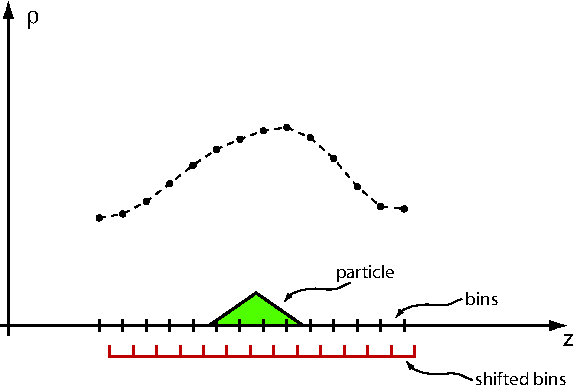
\includegraphics[height=8.4cm]{csr-bin.pdf}
\caption[CSR Calculation]
{The Coherent Synchrotron Radiation kick is calculated by dividing
longitudinally a bunch into a number of bins. To smooth the computed
densities, each particle of the bunch is considered to have a
triangular density distribution.}
\label{f:csr.bin}
\end{figure}

User settable parameters pertenent to the CSR simulation are listed in
\sref{s:csr.params}. Details of how the tracking is implemented is covered
in \sref{s:csr.track}.

\bmad simulates coherent synchrotron radiation using the formalism developed by
Sagan\cite{b:csr}. The total kick received by a particle is divided into two parts: The
space charge (SC) part and the coherent synchrotron radiation (CSR) part. \bmad further
subdivides the SC kick into longitudinal (LSC) and transverse (TSC) parts. Notice that
since the CSR kick is calculated using a 1-dimensional formalism, the CSR kick is strickly
lonitudinal. By definition, the LSC component is the kick that would result if all
particles were traveling in a straight line. The CSR component is what is left when the
LSC kick is subtracted off from the total kick. Generally, the LSC kick is negligible
compared to the CSR kick at large enough particle energies.

Transport through a lattice element involves a beam of particles. The lattice element is
divided up into a number of slices. Transport through a slice is a two step process. The
first step is to give all the particles a kick due to the CSR. The second step is
transport of all particles without any interaction between particles. Note that only the
longitudinal CSR kick is implemented and transverse kicks are ignored.

The particle-particle kick is calculated by dividing the bunch longitudinally into a
number of bins. To smooth the computed bin densities, each particle of the bunch is
considered to have a triangular density distribution as shown in \fig{f:csr.bin}.  The
particle density of a bin is calculated by summing the contribution from all the
particles. The contribution of a given particle to a given bin is calculated from the
overlap of the particle's triangular density distribution with the bin. For the CSR kick,
the density is actually calculated for a second set of staggered bins that have been
offset by 1/2 the bin width with respect to the first set. This gives the density at the
edges of the original set of bins. The density is considered to vary linearly between the
computed density points. For a description of the parameters that affect the CSR
calculation see Section~\sref{s:csr.params}.
 
